 % gjilguid2e.tex
% V2.0 released 1998 December 18
% V2.1 released 2003 October 7 -- Gregor Hutton, updated the web address for the style files.

\documentclass[extra,mreferee]{gji}
%\documentclass[extra]{gji}
\usepackage{timet}

\title[Improving the small-scale physical modeling for seismic numerical methods]
	{Improving the physical small-scale modeling for seismic numerical methods}
  %{Refined experimental studies for improving the reduced-scale physical modeling of seismic subsurface measurements}
\author[D. Pageot \textit{et al.}]
  {Damien Pageot$^{1,2}$, Donatienne Leparoux$^1$, Mathieu Le Feuvre$^1$, Olivier Durand$^1$ \and Philippe C\^ote$^1$ and Yann Capdeville$^3$ \\
  $^1$ G\'eophysique et \'Evaluation Non Destructive, IFSTTAR, Bouguenais, France. Email: damien.pageot@ifsttar.fr \\
  $^2$ Observatoire des Sciences de l'Univers Nantes Atlantique, Nantes, France. \\
  $^3$ Laboratoire de Plan\'etologie et G\'eodynamique de Nantes, CNRS, Universit\'e de Nantes, Nantes, France \\
  }
\date{Received 2016 xxxx; in original form 2016 xxxx}
\pagerange{\pageref{firstpage}--\pageref{lastpage}}
\volume{xxx}
\pubyear{2016}

\let\leqslant=\leq

\newtheorem{theorem}{Theorem}[section]

\newcommand{\psm}{small-scale physical modeling method}
\newcommand{\bialt}{\textit{BiAlt} }
\newcommand{\cmnt}[1]{}

\usepackage{soul}

\usepackage[dvipsnames]{xcolor}

\usepackage{lineno}
\usepackage{graphicx}
\usepackage{color}

\begin{document}

\linenumbers

\label{firstpage}

\maketitle

\begin{summary}
The potential of experimental seismic modeling at reduced scale has been explored for several years because it provides an intermediate step between numerical tests and geophysical campaigns on field sites. The MUSC device is an experimental bench that uses laser interferometry for recording ultrasonic data. It is a reliable tool able to produce experimental seismic reduced scale data from setups involving multisource and multireceiver positions. The recorded signals contain the complete seismic field, suitable for high-resolution imaging techniques like Full Waveform Inversion (FWI). However, experimental seismic modeling uses a point-source and generates 3D seismic data, whereas most wave propagation and imaging algorithms make use of 2D forward modeling for numerical cost reasons. Furthermore, geometrical spreading corrections applied to 3D data become limited in accuracy when geological structures are complex. This leads to inaccurate relative amplitudes between wavefronts which can have a significant impact on the quality of the parameters in the model. High-resolution imaging methods like FWI are also sensitive to the source waveform: in order to get reliable results, the initial synthetic source must be close enough to the true one, as in the case for the initial model. During the inversion process, the source wavelet can be estimated, either per shot or for the whole dataset, but it remains strongly dependent on the initial model, as this estimation will accommodate the discrepancy between the true and current model. In this paper we aim to demonstrate the potential of experimental seismic modeling for generating reproducible, realistic and suitable data which can be used as a reference for the validation of 2D high-resolution imaging methods. First, we refine the comparison between numerical and experimental data by generating accurate experimental line-sources, avoiding the necessity of geometrical spreading correction for 3D point-source data. In comparison with 2D and 3D numerical modeling based on the Spectral Element Method (SEM), we show the relevance of this approach with respect to published 3D correction methods, in particular when all seismic arrivals are taken into account. Second, we assess the experimental reproducibility of the source emitted in a model by the piezoelectric transducer during a MUSC campaign involving multisource multireceiver acquisition. Both these results refine the accuracy of experimental seismic modeling, and demonstrate that ultrasonic measurement benches allow the quantitative reproduction of the seismic wavefield generated by a hammer source. 
\end{summary}

\begin{keywords}
Controlled source seismology; Body waves; Surface waves and free oscillations; Wave propagation.
\end{keywords}

% ## INTRODUCTION
\section{Introduction}

% #### Nature and scope of the problem

Since the early developments of seismic imaging methods in the middle of 20th century, several approaches and algorithms have been proposed. The improvements of this last decade have focused on both qualitative imaging techniques such as migration (e.g., \cite{berkhout2012mss,guofeng2013gpu}), novel applications of quantitative imaging methods such as first arrival tomography (e.g. \cite{bohm2015cws}), and even more recent approaches like Full Waveform Inversion (e.g. \cite{perez2014awi}, see \cite{virieux2009fwi} for a review of the last decade). These refinements are proposed at different scales of application, from near-surface civil engineering structures to global crustal imaging, and include oil prospection. Validation is generally done using well-known shared benchmarks like the Marmousi model (\cite{martin2006marmousi2}). However, the synthetic data are generally computed using the same wave propagation modeling engine used in the inverse problem process. This approach is particularly useful for validating an algorithm in its early development stage but does not take into account the artifacts associated with the assumptions of the forward problem. On the other hand, it is often challenging to assess the accuracy of a given method on the basis of real experiments, in which precise information on the Earth's interior is absent and possibly leads to geological misinterpretation (\cite{morozov2004arf}). In this context, controlled experimental measurements appear to be a powerful intermediate step, provided they are capable of producing accurate data.

Small-scale physical modeling methods have been used for several decades to study the propagation of waves in media presenting different levels of complexity, ranging from acoustic wave propagation in homogeneous media to elastic wave propagation in 3D heterogeneous anisotropic media. This experimental approach was first used to describe the phenomenology of propagating waves (for example \cite{rieber1936ewp,howes1953sms,oliver1954two,angona1960two,obrien1971model}). Small-scale physical modeling was then used to test imaging processes (\cite{hilterman1970tdm,french1974mrp,bishop1985lvm,pratt1999fwi,mo2015development}), and validate numerical tools (\cite{favretto2013nmt}). The technology used for these different works has become increasingly sophisticated. Nowadays, most experimental benches include piezoelectric transducers to simulate multisources and multireceivers (\cite{wong2009spm}) or immersed zero-offset profiles (\cite{favretto2013nmt}). Laser interferometry is a recent alternative, providing seismic records free of coupling effects in solid media (\cite{bodet2005swi,vanwijk2006eir,bretaudeau2011ssm,bretaudeau2013fwi}) and in gel (\cite{decaqueray2011ewi}). All the above studies have shown the relevance of experimental seismic data obtained under controlled conditions. However, key points need to be addressed in order to quantitatively simulate seismic surface measurements generated with a hammer fall source: first, modeling surface waves prevents the use of immersed media (in which case it would be interface waves), and second, the omni-directionality of the radiation pattern of P-waves implies a physical source point. To this end, the MUSC (Mesures Ultrasonores Sans Contact in French) system has been designed (\cite{bretaudeau2011ssm}) to simulate: (1) wide-angle on-shore acquisitions, modeling both body waves and surface waves; (2) automatic multisource-multireceiver measurements with high-productivity, (3) high-precision source-receiver positioning; and (4) high-precision recording of absolute surface displacement without coupling effects. 

These abilities have been validated experimentally on a small-scale model containing a cavity (\cite{bretaudeau2011ssm}). The comparison with 2D numerical modeling showed close similarities on the diffracted and converted arrivals, after accounting for the experimental source waveform. Since the numerical source was simulated in 2D, some corrections were required to compare the resulting amplitudes, leaving moderate discrepancies that are discussed in \cite{bretaudeau2011ssm}. 

Our global objective here is to complete the validation of the capability of ultrasonic devices to precisely and quantitatively simulate surface seismic data carried out with multisource and multireceiver settings. This quantitative refined approach will increase the potential of the MUSC laboratory as a reliable tool for generating experimental data which will be distributed to the scientific community and used as references for validating seismic imaging methods. It is tackled through two experimental studies focusing respectively on two critical points : the 2D source emission and the effective source wavelet estimation. The first point is based on the following observations. 

At present 3D elastic wave propagation modeling methods are computationally expensive (\cite{etienne2010computational,borisov2013efficient,brossier2013performances,butzer20133d,borisov2015three}) and imaging methods are used mainly for 2D structures (\cite{brossier2009two,romdhane2011shallow,bretaudeau2013fwi,groos2014role}). Therefore forward problems implicitly use line-sources in 2D-space while field and experimental data are acquired using punctual sources that produce 3D wavefields. Consequently, the differences between 2D and 3D propagated wavefields must be explicitly taken into account to successfully validate imaging methods using field or experimental data.

To this end, a widely used method consists in spreading transformations of 3D-wavefields for 2D-media as a pre-processing step (\cite{crase1990robust,shipp2002two,ravaut2004multiscale,wang2009reflection,bretaudeau2013fwi}). Several 3D-to-2D transformation techniques have been proposed, each under the assumption that the medium is either 1D, or 2D but invariant along the axis perpendicular to the direction of the receiver-profile.

Recently, \cite{Forbriger_LSS_2014} and \cite{schafer2014lss} proposed the \textit{hybrid} method which makes it possible to correct geometrical spreading with good accuracy for both near- and far-field data, as recalled further on, but it is still an approximation and this method is known to fail to retrieve backscattered wavefield.

Thus, an ideal way to validate imaging methods is to work with 2D experimental dataset in controlled environment, \textit{i.e.} generated by a 2D source. We propose here to produce this data through an alternative path that consists in carrying out measurements from a source-line and making comparisons between numerical and experimental data following correction using the hybrid method. This approach constitutes the first study presented in te paper.

Another critical point for high-resolution imaging methods is knowledge of the source time function, generally treated as an unknown parameter in the case of field data. Good approximation of the source excitation allows avoiding source wavelet estimation during the inversion process and facilitating the validation of the imaging method. This source time function is estimated easily from experimental data, further supporting the use of small-scale physical modeling method for validating seismic imaging methods.

In this aim, the second study presented here consists in identifying the reproducibility of the source impact and thus data repeatability, and in estimating source time functions usable for 2D imaging methods.

Before the presentation of each experimental study, the specificities of the MUSC laboratory are explained in the first part below, followed by the presentation of the models used. Afterwards, the numerical characteristics of the code used are described. Several issues are dealt with here: (1) line-source versus point-source modeling, (2) validity of geometrical spreading correction, (3) reproducibility of the experiments and (4) the transducer influence on experimental data. These points are treated in two coupled studies on experimental data with the respective aims of: (A) refining the comparison between numerical and experimental data by taking into account the geometrical spreading effects between 2D and 3D data using an alternative approach (items 1 and 2), and (B) identifying the reproducibility of the source impact to validate data reproducibility (items 3 and 4).

These approaches will complete knowledge of the system and facilitate the achievement of massive multisource and multireceiver data simulating subsurface seismic experimental campaigns. Moreover, they provide quantitative information on data quality for geophysicists who need to use measurement-based data on reduced scale models. 

% ## METHODS
\section{Methods}

% #### MUSC bench
\subsection{Physical modeling: MUSC laboratory}

The MUSC laboratory (\cite{Bretaudeau_SSA_2008b,bretaudeau2011ssm,bretaudeau2013fwi}) has been built to experimentally reproduce low noise field seismic data on reduced scale models. Fig. \ref{Fig:Fig01} shows the measurement bench and its components: it is composed of a honeycomb tab and two arms that control the source and the receiver positions with a precision of 10 $\mathrm{\mu m}$.

The receiving system of the MUSC laboratory is a laser interferometer based on the phase shift of the reflected laser signal due to the particular displacement at the surface of the model during seismic wave propagation in the medium. The diameter of the laser beam on the model surface is 20 micrometers for a focal distance of 40 mm and makes it possible to detect a vertical displacement of the order of a nanometer in the frequency range of 10 kHz to 20 MHz. The laser interferometer constitutes a non-coupled receiver which avoids complicated modeling of coupling effects on measurements. The accuracy limits due to the laser beam size and the position precision will be discussed in a following part concerning the characteristics of the scale model tested. Thus, they will be assessed depending on the propagated wavelength in the case of a typical reduced scale configuration which is presented in this paper.

The seismic source in the MUSC laboratory is simulated by a piezoelectric transducer linked to a launching and synchronization system. It allows choosing the source function, i.e. a waveform like a Gauss or Ricker function, for a central frequency $f_{0}$ and a time delay $t_{0}$. To do this, the source is generated by a waveform generator and then amplified before being transmitted to the reduced-scale-model. The piezzo-electric transducers used are built to be adapted to the impedance of the resin model described in the next part. Thus the emitted signal, already presented in (\cite{bretaudeau2011ssm}) is not resonant. However, the sensor response combined with the coupling effect to the model behaves as a filter for the source shape. This effect is a crucial point that has been firstly tackled in MUSC by (\cite{bretaudeau2011ssm}) with an assumption of 2D propagation although it was done in case of a punctual source. In the present paper, we propose to study further the impact of this source response on the data by taking into account the 3D effects of a punctual source and by simulating a 2D source line. Note that the transducer response and the coupling effect depend on the frequency of the emitted signal. We will tackle this frequency dependance by taking into account the entire waveform of the pulse. \textbf{2D small-scale seismic laboratory exist (\cite{oliver1954two,angona1960two,mo2015development}) and have several advantages compared to 3D laboratory: (1) the variety of materials which can be anisotropic and which are less expansive and easier to handle contrary to sometime huge 3D epoxy-resin models or (2) much less source energy requirement (\cite{oliver1954two,mo2015development}). However, this method is based on the propagation of pseudo-longitudinal waves which are, in fact, non-dispersive Lamb waves while 3D methods propagate the full wavefield through the model without proxy for propagation velocities and wavetypes. More, 3D methods are best suited to reflection, refraction and diffraction problems than 2D methods (\cite{angona1960two}) which are critical in high-resolution seismic imaging.}

%Since the wave equation is linear
For the linearized wave equation, the change of scale must conserve the relationship between observables, i.e. amplitudes and time arrivals. Regarding the amplitude, the quality factor $Q$ is chosen to be in the same range as the materials of the near surface. The key parameter for the time scaling is the ratio between the propagated seismic wavelength and the spatial dimensions of the experiment, which include the model’s geometry, the spatial increment between the sources and the receiver positions, as well as the dimensions of the source impact. In the framework of seismic physical modeling, the latter must be as close as possible to a point source in order to simulate the spatial energy radiation pattern of a weight drop on the surface, i.e. with an omni-directional emitted P-wave. Actually, as explained in (\cite{bretaudeau2011ssm}), classical piezzo-electrical transducers sizes are generally large compared to the emitted wavelength and provide a directional emission pattern for P-waves whereas a hammer fall source used in subsurface field measurements behaves as a punctual impact and provides an omnidirectional emission pattern of P-waves. For this reason, in the MUSC laboratory, two adapted sources have been tested in term of directivity pattern by (\cite{bretaudeau2011ssm})  who showed their capacity to simulate a thin piston effect. For the spectral band [20 kHz; 200 kHz], a commercial piezoelectric transducer is used without any coupling gel. For the spectral band [300 kHz; 800 kHz], the piezoelectric source is coupled through a conical adapter stuck to the transducer to obtain the expected impact surface. The resulting radiation patterns of the sources are constantly quasi-omnidirectional for P-waves in the range of the frequencies recorded (see \cite{bretaudeau2011ssm} for details). 
These two frequency bands, called here "lower frequency band" and "higher frequency band", have been chosen to allow both complying with the dimensional scale ratio presented in Tables 1 and 2 and making easily the heterogeneities in the medium. That means : the heterogeneities should be not too small (1mm of minimal size) and the total model size should not be too big or too heavy (1m2 and 270 Kg max) for the supporting table. For simulating seismic experiments applied to the near surface , we use preferentially the low frequency band which allows a dominant wavelength (at 100kHz) about 13 mm for the Rayleigh waves and 28 mm for the P waves, by taking into account the velocity in the models described in a following part. The scale ratio rules used are summarized in Tables 1 and 2. In the first case (Table 1), a central frequency of 100 kHz in the laboratory corresponds to a central frequency of 100 Hz in the field, whereas in the second one (Table 2) a central frequency of 100 kHz in the laboratory corresponds to a central frequency of 50 HZ in the field. Note that with these propositions, the quality factor $Q$ and the density $\rho$ are modeled with a ratio equal to 1, i.e. they remain the same at both scales. Indeed, small scale models are generally made of thermoplastic or epoxy resin casting materials (\cite{bretaudeau2013fwi}).The mechanical properties of these materials provide attenuation characteristics close to those of the natural soil materials of subsurface media. Their seismic velocities are about twice those in subsurface materials, as proposed in Table 2. The possibilities of combinations can generate the impedance contrasts encountered in geophysical problems. 

The MUSC bench presented above has been designed to simulate typical subsurface seismic measurements of field campaigns with considerable reproducibility. The validation was performed by comparison between small scale measurements and numerical data (\cite{bretaudeau2011ssm}). The results have demonstrated the considerable reproducibility of the converted and diffracted events recorded on the vertical component. The amplitude analysis was performed with 2D-3D corrections but small discrepancies remained due to the difficulty of taking into account the S and P waves in the same way. Consequently, to avoid these discrepencies we propose here to refine the study by testing a more recent correction methodology \cite{schafer2014lss} and by providing experimental and numerical 2D and 3D data. This approach is achieved using the data with the two models presented below.

% ## Models
% ## Models
\subsection{Characteristics of the scale models tested}
\label{sec:models}

In this study, we consider two different reduced scale models. The first is homogeneous whereas the second one, called \bialt, contains a deeper layer with a geometrical variation of the interface along the profile. The top layer, as well as the entire first model, is made of epoxy-resin called F50 pure. The deeper layer is built with a denser resin called LAB1000. The specific properties of these two kinds of resins are summarized in Table 3 with other commonly used materials. Note that the Q-factor values are of the same order as the Q-factor value in the shallowest parts of certain natural media.

As described in the previous part and proposed in Table 2, it is possible to take into account a scale ratio equal to 2 between real and reduced model velocities. Thus, using a 100 kHz Ricker source will simulate a 50 Hz Ricker source in reality, which is realistic for simulating a hammer impact on a surface. In this case, the distance scale ratio is 1000, so a distance of 1 mm in the laboratory experiment corresponds to a distance of 1 m in reality. 

As mentionned before, the laser beam diameter used for recording the propagating waves is 20 $\mu$m wide. In the presented study, typical of experimentations in MUSC, the dominant wavelength (at 100kHz) equals about 13 mm for the Rayleigh waves and 28 mm for the P waves . Thus, the laser beam respectively equals  $\lambda /650 $ and $ \lambda /1400 $  . At the field scale, and following the rules in table 1, those correspond to measurement surfaces of 20 mm and 2 mm respectively. These dimensions are lower or equivalent to the possibilities available by geophones holds. Thus, at the laboratory scale in MUSC, the measurement accuracy in term of the size of the recording surface is respected.

In parallel, the position accuracy of the receiving system is 10$\mu$m. This value is lower to the focal beam. It corresponds to the center position of the laser beam, which is 20$\mu $m large. In practice, the incremental displacement between two receivers positions used generally equals 1 mm. It is higher than the focal beam size.

Furthermore, as shown on figure 2, even if the emission properties of a piezo-electric transducer is narrow-band, the spectral bandwith of the pulse emitted by the piezo-electric transducer is large enough to simulate a seismic pulse emitted by a hammer fall in subsurface media, through the scale ratio used in table 2: the frequency of 100KHz in MUSC corresponds to 50Hz at field scale and 150 KHz corresponds to 75 Hz.

In the next section, the recorded signals will be analyzed for a maximum offset equal to 60 mm in the case of the homogeneous model and 100 mm for the \bialt model. Thus the resin models have to be wide enough to accommodate this receiver-source distance without creating boundary echoes that could interfere with direct arrivals. To do this, the homogeneous model is 500 mm long, 504 mm large and 115 mm high. The \bialt model is 540 mm long, 300 mm large and 203 mm high. The geometry is presented in Fig. \ref{Fig:Fig03} and simulates an interface between a 3 m thick layer of clay over a limestone layer.

These two resin blocks and their corresponding numerical models will be used for generating seismic data with punctual sources and line sources for the homogeneous model, in order to study the effective source excitation emitted on the MUSC bench and its reproducibility.

% #### Spectral Element Method
\subsection{Numerical modeling: Spectral Element Method}

For this study we need a numerical modeling method whose spatial discretization is suitable for representing complex environments and which provides both high precision results and low numerical dispersion. Thus we use the Spectral Element Method (SEM) for two-dimensional and three-dimensional elastic wave propagation modeling (\cite{komatitsch1998spectral,komatitsch1999spectral,komatitsch2005spectral,Festa_PML_2005}). 

SEM is a variant of the Finite Element Method (FEM) (\cite{Lysmer_FEM_1972,Seron_FEM_1990,Hulbert_FEM_1990,Tromp_SEM_2008}) based on a high-order piecewise polynomial approximation of the weak formulation of the wave equation which leads to a spectral convergence ratio as the interpolation order increases. Considering near-surface experiments, one advantage of SEM is that the weak formulation naturally satisfies the free-surface condition used to simulate surface wave propagation with considerable accuracy (\cite{komatitsch1998spectral,komatitsch1999spectral,komatitsch2005spectral}). Contrary to FEM, which calls on a wide range of available element geometry (\cite{dhatt1984finite}), SEM is limited to quadrilateral elements in 2D and hexahedral elements in 3D. Note that although SEM with tetrahedral elements exists (\cite{komatitsch2001wave}) it leads to theoretical complications. However, quadrangles and hexahedra are well suited for handling complex geometries and interface matching conditions (\cite{Cristini_SEM_2012}). 

In SEM, the wave-field is expressed in terms of high-degree Lagrange interpolants and the calculations of integrals are based on the quadrature of Gauss-Lobatto-Legendre (GLL). Each element is discretized with Lagrange polynomials of degree $n_{l}$ and contains $n_{l}+1$ GLL points that form its local mesh. This combination of high-degree Lagrange interpolants with the GLL integration leads to a perfectly diagonal mass matrix which in turn provides a fully explicit time scheme suitable for numerical simulations on parallel computers (\cite{komatitsch1998spectral,komatitsch1999spectral}).

The spatial resolution of SEM is controlled by the typical size of an element ($\Delta h$) and the polynomial degree in use on an element ($n_{l}$). Typically, a polynomial degree $n_{l}=4$ is optimal for seismic wave propagation modeling (\cite{moczo2011finite}) although $n_{l}=8$ remains numerically affordable in 2D. To obtain accurate results, the required $\Delta h$ is of the order of $\lambda_{min} /2 < \Delta h < \lambda_{min}$ for $n_{l}=4$ and $\lambda_{min} < \Delta h < 2\lambda_{min}$ for $n_{l}=8$, $\lambda_{min}$ being the smallest wavelength of the waves propagated in the model. The time marching scheme is governed by the CFL stability condition:

\equation
\Delta t < \mathcal{C}\frac{\Delta h}{c_{max}}\,
\endequation

where $\mathcal{C}$ is the Courant constant and $c_{max}$ is the maximum wave velocity, typically the P-wave velocity. The Courant constant $\mathcal{C}$ is determined empirically, depending on the application, and is fixed at a maximum of 0.30 for this study.

The numerical meshing required for the numerical simulations involves cell dimensions of about $e_{s}<3.43\ mm$ for the F50 material and $e_{s}<4.66\ mm$ for the LAB1000 material, considering a polynomial degree $n_{l}+1=5$ and a slightly over-estimated maximum frequency of $f_{max}=300\ kHz$ for $f_{0}=100\ kHz$. In our study, the models are meshed with quadrangles (2D) and hexahedra (3D) using the GMSH open-source software package (\cite{Geuzaine_MSH_2009}).

% #### From point-source to line-source acquisition
%\subsection{From point-source to line-source response}
\section{From point-source to line-source response}

The approach described here consists in generating data with a 3D constructed line-source (equivalent to numerical 2D point-source modeling) as well as a 3D point-source and analyzing the similarity with numerical results under the same conditions. This is done to respond to two needs: 1) the quantitative refined validation of the reduced scale data, 2) the capacity of the reduced scale bench to generate 2D data sets that are intermediate between numerical simulation and field data suitable for the 2D imagery tests. Indeed, in the framework of wave propagation modeling and imaging methods, although 3D acoustic algorithms exists (\cite{benhadjali_FWI_2008,plessix_FWI_2010}) and 3D elastic algorithms are still being developed (\cite{castellanos_AMD_2011,borisov2015three}), most available algorithms are limited to 2D elastic and 3D acoustic approximation, mostly due to reasons of computational cost. Furthermore,  validation of the inversion process is often limited to processing made with synthetic data using the same model for computing both predicted and estimated measurement, while the validity of applications on real datasets is conditioned by good \textit{a priori} and poor knowledge of the target. All of these lead to a limited validation of the efficiency of imaging methods to recover parameter models. Thus accurately correcting the difference between 2D and 3D geometrical spreading is critical for the 2D inversion of field data.

Many strategies exist to correct geometrical spreading effect differences between 3D and 2D data, the two widely used are (1) data convolution with $\sqrt{t^{-1}}$ together with the application of a $\sqrt{t}$ taper function (\cite{crase1990robust,shipp2002two,ravaut2004multiscale}) and (2) data tapering ($\sqrt{t}$) and inference of a source function by linear inversion to estimate the correct the phase (\cite{pratt1999fwi,bretaudeau2013fwi}). However, these strategies are used to transform data which contains essentially body waves (except \cite{bretaudeau2013fwi}) and the first one is known to produce artefacts which can be significant (\cite{auer2013critical}). To overpass these limitation and transform near-surface data dominated by surface wave, \cite{Forbriger_LSS_2014} have recently developed the \textit{hybrid} method and validate it through numerical tests (\cite{schafer2014lss}).

The \textit{hybrid} method presented in the appendix is an efficient spreading transform which makes it possible to reconstruct velocity models with the 2D-FWI method using 3D-data. However, this method is derived from a far-field acoustic approximation of Green's functions and is known to fail for back-scattered surface waves (\cite{schafer2014lss,groos2014role}). Moreover, the correct smooth transition between \textit{single-velocity} and \textit{direct-wave} transformations, which are the two components of the \textit{hybrid} method, is not easy to determine without 2D reference data. This is the case for both field and experimental data and the spreading transformation results become strongly dependent on the user's attempts, expertise and know-how.
Thus the missing step between purely numerical validation and real data applications can be addressed by an alternative approach that consists in recording experimental seismograms generated by line-sources under controlled conditions. Here, we take advantage of the experimental framework to explore this alternative approach specific to the MUSC laboratory, \textit{i.e.} by carrying out 2D measurements from 3D constructed line-source. Fig. \ref{Fig:Fig05} shows a schematic representation of the principle of this kind of experiment. The line-source is composed of a finely-sampled line of point-sources and a line of receivers for each offset considered. 

% \textbf{Note that 3D constructed line-source response corresponds to the wavefield generate by a line source in a 3D space}
For practical reasons in the MUSC laboratory, the experiment is carried out through the principle of reciprocity in the case of recording a vertical source and a vertical component, with one source position and a set of receiver positions spread out along the invariant direction. For each source position (i.e. for each offset), all traces of each set of receivers are then stacked together to obtain the 3D constructed line-source response. In order to apply this protocol, we choose a suitable sampling interval $\Delta s$ between each point-source constituting the pseudo line-source to ensure the applicability of \textit{Huygens principle}. Given the material properties of $F50\ pure$ epoxy-resin, we choose an interval $\Delta s=\lambda_{min}/10 \tilde{=}0.5\ mm$ over a line of $300\ mm$ long which leads to 601 point-source positions.

Four receiver positions are available: 45, 50, 55 and 60 mm offset. The source time function (for the numerical simulation as well as for the experimental test) is a Ricker wavelet, the second derivative of a Gaussian function:

\equation
s(t) = (1-2(\pi f_{0}(t-t_{0}))^{2})~e^{-(\pi f_{0}(t-t_{0}))^{2}}~,
\label{eq:ricker-source} 
\endequation

where $f_{0}$ is the central frequency and $t_{0}$ is the peak time. Here, we take a central frequency $f_{0}=100\ kHz$ and $t_{0}=0.03\ ms$. The data sets obtained are filtered using a low-pass Butterworth filter with a cutoff frequency $\omega_{c}=250\ kHz$ to remove noise and tapered at the beginning using a cosine taper function of width $w=0.03\ ms$ on the time signal. The 3D constructed line-source data is obtained through a weighted stack over common offset traces. Fig. \ref{Fig:Fig06} shows the results for both the numerical simulation and the experimental data. The signals emitted by a line of point-sources and recorded at the first receiver position (45 mm) are presented in Figs \ref{Fig:Fig06}(a) and \ref{Fig:Fig06}(c) for the numerical and experimental tests, respectively. Note that no attenuation is accounted for in the numerical modeling, so we do not compare the numerical and experimental results directly. Moreover, all the resulting traces are normalized to be comparable to the experimental tests. The numerical result (fig \ref{Fig:Fig06}(a)) clearly shows the attempted direct P and S wavefronts and the reflected PP and P-SV wavefronts, as mentioned previously (labels $1$, $2$, $3$, $4$ in Fig. \ref{Fig:Fig06}). These similarities between the numerical simulation and the experimental data are altered by multiple echoes visible on the experimental data (labeled E in Fig. \ref{Fig:Fig06}(b)), as a ringing effect on the source wavelet due to the piezoelectric transducer coupling on the model surface. This point will be addressed in the next section which focuses on source reproducibility. 

Figs \ref{Fig:Fig06}(b) and \ref{Fig:Fig06}(d) present the comparisons of 3D point-source (red line) and 3D constructed line-source (green line) data at the first receiver position (45 mm offset) for the numerical and experimental tests, respectively. To complete the comparison, a 2D modeling result is added in Fig. \ref{Fig:Fig06}(b) (gray line) as a reference.

Fig. \ref{Fig:Fig06}(b) shows that the 3D constructed line-source data (green line) provided with a set of punctual sources is perfectly superimposed on the 2D reference data (blue line) until 0.18 ms. Afterwards, the PSv amplitude (\textit{i.e.} the last arrival) is abnormally high for the sampled line-source data. As shown in eq. \ref{eq:line-point-relation}, a line-source is a sum of an infinite number of point-sources along an axis. Here, the finite dimensions in space of the experimental 3D setup can cause boundary effects and thus this difference in amplitude.

For the earlier arrival, the global fit between the numerical data highlights the validity of sampling a finite line-source by a set of point-sources. Concerning both the numerical (Fig. \ref{Fig:Fig06}(b)) and experimental (Fig. \ref{Fig:Fig06}(c)) cases, the comparison of 3D point-source and 3D constructed line-source data shows the expected phase shift of $\pi/4$ (see appendix eq. \ref{eq:far-field-frac}). Similar comparisons for the four source-receiver offsets are shown in Figs \ref{Fig:Fig07}(a) and \ref{Fig:Fig07}(c) for numerical and experimental data, respectively.

To test the improvement of our approach to provide line-source data in comparison to spreading transformation methods, our results are compared to data obtained using the \textit{hybrid} method. Figs \ref{Fig:Fig07}(b) and \ref{Fig:Fig07}(d) present the comparison between the 3D constructed line-source data acquired from a set of punctual sources (green line) and transformed 3D point-source data (blue line). The comparison of numerical results (Fig. \ref{Fig:Fig07}(b)) shows that the \textit{hybrid} method is able to produce equivalent line-source data with very good agreement in terms of both amplitude and phase for direct arrivals. However, PP and PSv reflected waves (back-scattered wave) remain different. The same comparison is made for the experimental data in Fig. \ref{Fig:Fig07}(d). This last result also shows good agreement between line-source and transformed point-source data up to 0.12 ms (mainly direct-waves). However, discrepancies occur for the reflected waves. The first reflected wave is marked by a red line in Figs \ref{Fig:Fig07}(b) and \ref{Fig:Fig07}(d).

These disagreements are more marked than in the numerical case: the correction of the geometrical spreading with the hybrid method seems unable to correctly scale the amplitude due to interference from the echoes of the source and reflected wave. Consequently, a 3D constructed line-source should be recommended instead of the hybrid correction of data to take into account all the seismic arrivals. Concerning the signal recorded at the $55\ mm$ offset, the largest difference in amplitude can be explained by a weaker \textit{signal-to-noise} ratio than for the three other offsets in the experimental data. 

These results obtained using our approach to generate 3D  experimentally constructed line-source data show that the MUSC laboratory is efficient and can produce reliable experimental 2D data suitable for migration-based methods such as 2D-FWI. Thus it plays the role of an intermediate tool capable of providing 3D point-source and 3D constructed line-source data without the need for geometrical spreading corrections.

% #### Experimental source reproducibility
%\subsection{Experimental source reproducibility}

\section{Experimental source time function}

In the framework of high-resolution imaging, such as FWI, the first validations of the method are generally performed with synthetic data generated with the same modeling engine than the one used for inversion. In these cases, the source waveform is known and the initial model $m_{0}$ is generally a smoothed version of a known true model used in the forward problem to obtain synthetic observed data. Consequently, no source wavelet estimation is necessary. However, obtaining knowledge of the original source time function is an important task when real data are inverted. The solution of the source is obtained using a linear source wavelet estimation (\cite{pratt1999fwi,virieux2009fwi}) which can integrate all the data from multisource/multireceiver acquisition and the estimated source excitation is given by:

\equation
S_{est}(\omega)=\sum\limits_{i=1}^{N_{S}}\sum\limits_{j=1}^{N_{R}}\frac{H_{ij}(\omega)G_{ij}(\omega)^{*}}{H_{ij}(\omega)H_{ij}(\omega)^{*}}S(\omega)\ ,
\label{eq:lswe}
\endequation

where $\omega$ is the angular frequency, $S_{est}$ is the real Fourier transform of the estimated source, $G(\omega)$ is the real Fourier transform of the observed signal, $H(\omega)$ is the real Fourier transform of the signal calculated in the synthetic model, $S(\omega)$ is the synthetic source used to compute $H(\omega)$, $N_{S}$ is the number of sources, $N_{R}$ is the number of receivers and $^{*}$ denotes the conjugate. The main issue of this method is that inaccuracies in the synthetic model, and consequently in the calculated data, are integrated in the estimated source. The resulting distortion of the estimated source wavelet can lead to inaccuracies in the updated models during data inversion and then in the recovered parameters of the final model. Moreover, for a given dataset, one or more specific sources need to be estimated, depending on whether the source is considered stable enough from one shot to another or not. However, estimating the source for each shot in the case of numerous multisource/multireceiver data can lead to significant additional numerical cost. Thus knowledge of the source time function and its stability are two crucial key points in modeling experimental data for testing imaging processes.

We showed in the previous section that the MUSC laboratory is able to generate high quality experimental 3D constructed line-source seismograms. If the source waveform is constant during a multisource-multireceiver experiment, it will be very efficient for validating the imaging method. As shown by \cite{bretaudeau2011ssm}, the source waveform injected into the reduced-scale model by the piezoelectric source is different from the selected theoretical one. Indeed, Figs \ref{Fig:Fig06}(c) and \ref{Fig:Fig06}(d) show multiple wavefronts following that of the first arrival. These multiple echoes are due to the coupling of the piezoelectric source on the material. This can depend on the material as well as the force applied on the transducer and naturally raises the question of the ability of the MUSC laboratory to provide reproducible sources during a complete multisource/multireceiver experiment. In order to evaluate the reproducibility of the source impact, several numerical and physical models described below were applied to the same \textit{F50 pure} homogeneous epoxy-resin block as in the previous section.

In the first step, ten events were acquired for this model with a similar geometrical setup: 120 receiver positions with an increment of $\Delta r= 1\ mm$ and a minimum source-receiver offset of $r=10\ mm$ (see Fig. \ref{Fig:Fig08}). The numerical wavelet sent to the piezoelectric transducer source is a Ricker function with a central frequency of $100\ kHz$ and $t_{0}=0.03\ ms$. Each data set is filtered using a low-pass Butterworth filter with a cutoff frequency of $\omega_{c}=250\ kHz$ to remove noise and tapered at the beginning using a cosine taper function of width $w=0.03\ ms$. Then, a 3D/2D geometrical spreading correction is applied using the \textit{hybrid} method. As shown previously, this correction is well adapted for correcting direct arrivals which are preferentially taken into account to determine the source wavelet. Fig. \ref{Fig:Fig09} shows the resulting central trace ($r=70\ mm$) of each realization (red line signals) compared to a reference central trace resulting from the average of traces for the same offset (signal indicated by a green line). The good agreement between the central traces and the reference signal is the first validation of the reproducibility of the source in the same experiment. This agreement is strengthened by a correlation coefficient higher than $0.98$ in each case. To go further in this comparison, a mean correlation coefficient, for all the traces, is calculated for P-, S- and PP-waves. The mean correlation coefficients for S- and PP-waves are closed to the maximum ($0.99$) and confirmed the good agreement between traces for these phases. For the P-wave, the mean correlation coefficient is smaller ($0.84$) but still good. This last can be relied to the signal-to-noise ratio which can vary from an experiment to an other and impact mostly the P-wave as it can be seen on shot $10$ (Fig. \ref{Fig:Fig09}).

In the second step, a unique source wavelet is estimated using eq. \ref{eq:lswe}. As done previously, the signals are normalized to avoid the intrinsic attenuation effects on the direct arrivals. The source wavelet estimation takes into account the vertical components of the ten experiments together and allows obtaining a mean effective source time function (Fig. \ref{Fig:Fig10}). This effective source is very different from the theoretical one, with strong asymmetry around the main peak at $t_{0}$ and a long sequence of source echos from $t=0.04\ ms$ to the end of the time window. This source wavelet, convolved with all the synthetic signals, should reproduce the experimental data if the real source wavelet is the same for all the experiments. The resulting traces are presented in Fig. \ref{Fig:Fig10}(b), which shows that the corrected synthetic seismograms are in good agreement with the experimental ones, with a correlation coefficient higher than $0.92$ in each case. These correlation coefficients are not as good as the previous ones. This can be explained first by the fact that the 3D-2D geometrical spreading correction applied to the experimental traces is not fully efficient for later arrivals, and second because we neglected the effects of quality factors. Consequently, the estimated source is close to the real one but contains the inaccuracies from both the numerical modeling and the geometrical spreading correction. Again, we estimate mean correlation coefficients for P-, S- and PP-wave and note the good agreement for S- and PP-waves. However, the mean correlation coefficient for the P-wave is quite low ($0.64$). Indeed, in addition of the signal-to-noise ratio, the potential inaccuracies of the numerical model (P-wave and S-wave) and the absence of intrinsic attenuation strongly impact the source estimation.

However, these latter results based on an average estimated source wavelet show that the source time function emitted by the transducer in the MUSC laboratory measurement bench is stable enough to ensure robust source reproducibility for a complete physical experiment with multiple source and receiver positions. Therefore, concerning the key issue of source data, the experimental data acquired in the MUSC laboratory can be efficiently processed by imaging methods such as Full Waveform Inversion (FWI) with only one estimation step for all the multisource and multireceiver data.

\section{Application to complex model}

In the previous approaches developed for the geometrical spreading correction calibration and the source estimation, the studies were performed on a homogeneous block of F50 epoxy-resin. This approach facilitates developments and applications but limits the validation to a simple medium with a simple acquisition geometry. Thus here we consider a more complex model called \bialt (see section \ref{sec:models} for description). The acquisition setup is composed of shots with 241 receivers spaced by $\Delta r=0.5\ mm$. The receiver line 120 mm long is centered on the medium axis, where the topography of the 2-layer interface provides a valley-shape curve layout for which 25 source positions are considered, ranging from 0 to 241 mm with a spacing of $\Delta s=10\ mm$. The source wavelets are modeled by a Ricker function with a central frequency equal to $f_{0}=75\ kHz$ and parameter $t_{0}=0.03\ ms$. A low-pass Butterworth filter ($\omega_{c}=200\ kHz$) and a cosine taper are applied to the data. Given that the top layer of the model is made of the same epoxy-resin as for the homogeneous block, we applied the hybrid geometrical spreading correction with the same parameters. The corresponding synthetic data were generated using a 2D SEM algorithm. Again, the quality factor is not taken into account. Fig. \ref{Fig:Fig11}(a) shows the effective source wavelet estimated from the $241 \times 25$ traces compared to the theoretical one. In this case, the estimated source wavelet seems more symmetrical than those recovered for the previous experiment. Moreover, few and very low amplitude multiple echoes occurred compared to the previous estimated wavelet. This could be related to the lower central frequency of the source which may generate fewer multiple reflections at the interface between the piezoelectric source and the surface of the material surface. Once again, this estimated source is convolved with the synthetic data and the resulting traces for the first source are shown in Fig. \ref{Fig:Fig11}(b) (blue line). The comparison between the experimental traces (black) and numerical traces computed with the Ricker source wavelet (red) shows that the relative amplitude between the P and S wavefronts are very different, in particular between the intermediate and far offset. The convolution with the estimated source provides good agreement between the experimental data and the numerical data and highlights the relevance of the source inversion for the imaging process. The residual discrepancies were due to the estimation of the quality factor of the epoxy resin \textit{LAB1000} that will be refined in further studies. Moreover, given that the effective source is estimated using a realistic multisource-multireceiver design with 25 source positions, these results confirm the stability of the source during large experimental campaigns. 


% ## CONCLUSIONS

\section{Conclusions}
 
High-resolution seismic imaging methods are mostly developed with 2D approximation and require real data to complete the validation of the inversion process often limited to processing made with synthetic data using the same model for computing both predicted and estimated measurement. We demonstrated here that the geometrical spreading and amplitude corrections usually used to transform 3D in 2D real seismic data are limited and can be replaced by accurate experimental 2D data recorded in a controlled environment. This alternative process was shown to be more accurate when taking into account all the arrivals, especially 
when ringing interfere with the direct arrivals.

In the second step, the effective source wavelet emitted in the material after the coupling effect of the transducer and its possible variability were studied. Given that knowledge of the source is an important aspect for certain seismic data inversion algorithms, source estimation is performed using the linear source wavelet estimation method which integrates the entire signal and is strongly dependent on the accuracy of the initial numerical model. It is preferable to have the same source wavelet throughout a complete experiment. Thus we studied the experimental source and validated its good reproducibility for multisource-multireceiver experiments in the case of a homogeneous medium and for a two-layer model having an internal interface with varied topography. The good repeatability of the source wavelet recovered and the high correlation coefficient of the simulated data in comparison to the experimental data, demonstrated the quality of the experimental data obtained using the MUSC reduced scale measurement bench. 
Thus these studies successfully improved the capacity of the physical model designed for seismic experiment simulation. 

Further studies will focus on quality factor estimation to avoid the normalization calculation in the process and provide several sets of perfectly controlled experimental data to the scientific community. Moreover, the study of effective source reproducibility will be extended to the horizontal component that has become available recently in the MUSC laboratory (\cite{valensi2015multicomponent}).

\begin{acknowledgments}
We would like to thank the reviewers for their valuable comments and suggestions to improve the quality of the paper.
We would like to thank the CEA for the SEM3D Spectral Element Method modeling code. We are also grateful to the CCIPL(Nantes, France) for providing access to its high-performance computing facilities and the support given  by its staff. Finally, this study was carried out within the framework of the VIBRIS project (OSUNA-IFSTTAR-CNRS) sponsored by the Pays-de-la-Loire Region (France). 
\end{acknowledgments}

\clearpage
\newpage

\bibliographystyle{gji}
\bibliography{GJInt2016}

\clearpage
\newpage

\section*{Annexe: 3D/2D differences}

In this appendix we shall describe 3D-2D spreading corrections proposed by \cite{Forbriger_LSS_2014}: \textit{single velocity}, \textit{direct wave} and \textit{hybrid} methods.

The displacement field $u$ can be evaluated at position $(\mitbf{x}=(x,y,z))$ and time $(t)$ by (\cite{aki2002quantitative}):

\equation
u(\mitbf{x},t) = \int_{-\infty}^{+\infty}d\tau \int \int \int_{V} G(\mitbf{\xi},t-\tau;\mitbf{x},0)f(\mitbf{\xi},\tau)dV(\mitbf{\xi})\ ,
\label{eq:displacement}
\endequation

where $G(\mitbf{\xi},t-\tau;\mitbf{x},0)$ is the Green's function between the source location $(\mitbf{\xi})$ and the observation point $(\mitbf{x})$ ; and $f(\mitbf{\xi},\tau)$ is the seismic source function. The body force distribution for a point source ($f_{P}$) and a line source ($f_{L}$), located at positions $ \mitbf{x_{s}}=(x_{s}, y_{s},z_{s}) $ and $ \mitbf{x_{s2D}}=(x_{s},z_{s}) $, respectively, in a 2D structure invariant along the y-axis are :

\equation
f_{P}(\mitbf{x},t;\mitbf{x_{s}})=\mitbf{F}(t)\delta_{\mitbf{x}}(x-x_{s})\delta_{\mitbf{x}}(y-y_{s})\delta_{\mitbf{x}}(z-z_{s})\ , \label{eq:point-force}
\endequation

\equation
f_{L}(x,t;\mitbf{x_{s2D}})=\mitbf{F}(t) C \delta_{\mitbf{x}}(x-x_{s})\delta_{\mitbf{x}}(z-z_{s})\ , 
\label{eq:line-force}
\endequation

where C is a constant, $(\mitbf{F}(t)) $ is the wavelet time function and $(\delta)$ is the Dirac function. Substituting eq. \ref{eq:point-force} in eq. \ref{eq:displacement} and eq. \ref{eq:line-force} in eq. \ref{eq:displacement} leads to the wave motion due to a point-source $u_{P}$ and the wave motion due to a line-source $u_{L}$ 

\equation
u_{P}(\mitbf{x},t;\mitbf{x_{s}})=\int_{-\infty}^{+\infty}\ G(\mitbf{x_{s}},t-\tau;\mitbf{x})F(\tau)d\tau, 
\label{eq:point-displacement}
\endequation

\equation
u_{L}(\mitbf{x},t;\mitbf{x_{s}^{2D}})=\int_{-\infty}^{+\infty} \int_{-\infty}^{+\infty} G(\mitbf{x_{s}^{2D}},t-\tau;\mitbf{x})F(\tau)Cdy'd\tau\ , \label{eq:line-displacement}
\endequation

The equivalent displacement $u_{L}$ for a line-source can be obtained by the displacement field $u_{P}$ generated by a point source by integration along $y$:

\equation
u_{L}(x,y,z,t;x_{s},z_{s})= \int_{-\infty}^{+\infty}u_{P}(x,y,z,t-\tau;x_{s},y',z_{s},0)Cdy'\ .
\label{eq:line-point-relation}
\endequation

Eq. \ref{eq:line-point-relation} shows that in terms of amplitude, the displacement generated by a line-source is greater than the displacement generated by a point-source.
Taking $g_{k}^{3D}(r)$ and $g_{k}^{2D}(r)$, the Fourier transform of the 3D and 2D Green's function in the acoustic approximation, respectively, with $k$ being the wavenumber and $r=|\mitbf{x}-\mitbf{x_{s}}|$ the source-receiver offset. In the far-field approximation, \cite{Forbriger_LSS_2014} demonstrate:

\equation
\lim\limits_{r \rightarrow \infty} \frac{g_{k}^{2D}(r)}{g_{k}^{3D}(r)}\approx \sqrt{\frac{2\pi r}{k}}.e^{i\frac{\pi}{4}}\ .
\label{eq:far-field-frac}
\endequation

Replacing the wavenumber $k=\omega/v_{ph}$, where $\omega$ is the angular frequency and $v_{ph}$ is the phase velocity, results in:

\equation
\sqrt{2\pi r v_{ph}}.\sqrt{\frac{\pi}{\omega}}e^{i\frac{\pi}{4}}=F_{amp}.\widetilde{F}_{\sqrt{t^{-1}}}\ ,
\endequation

where $F_{amp}=\sqrt{2\pi r v_{ph}}$ is the amplitude factor and $\widetilde{F}_{\sqrt{t^{-1}}}$ applies the phase shift. It results in:

\equation
u_{L}(r,\omega)=u_{P}(r,\omega).F_{amp}.\widetilde{F}_{\sqrt{t^{-1}}}\ .
\label{eq:single-velocity}
\endequation

This correction is called the \textit{single-velocity} transformation which is recommended, after numerical tests (\cite{Forbriger_LSS_2014, schafer2014lss}), for small offsets. For a larger offset, by stating that the offset is almost equal to the propagation distance, \cite{schafer2014lss} propose to replace the previous amplitude factor with:

\equation
\label{eq:direct-wave}
F_{amp}=r\sqrt{\frac{2 \pi}{t}}\ .
\endequation

The resulting correction is called the \textit{direct-wave} transformation. Finally, the \textit{hybrid} method proposed by \cite{Forbriger_LSS_2014} and \cite{schafer2014lss} consists in using the two previous transformations with a smoothly offset conditioned transition from the near-field to the far-field.

The \textit{hybrid} method was successfully validated by \cite{schafer2014lss} in numerical modeling and reconstruction tests with a 2D FWI method and 3D numerical data generated in a 2D structure. 


\clearpage
\newpage

\begin{table}
\centering
\caption{ example of possible scale ratios between field experiments (FEx) and MUSC experiments (MEx) when considering a ratio equal to 1 for the density and quality factors.}
\begin{tabular}{cccccc}
\quad & FEx scale & MEx scale & scale ratios \\
P waves velocity & $\mathrm{V_{p 0}}$ & $\mathrm{V_{p 0}}$ & 1 \\
S waves velocity & $\mathrm{V_{s 0}}$ & $\mathrm{V_{s 0}}$ & 1 \\
Time & $\mathrm{T_{0}}$ & 0.001 $\mathrm{T_{0}}$ & 0.001 \\
frequency & $\mathrm{F_{0}}$ & 1000 $\mathrm{F_{0}}$ & 1000 \\
Distance & $\mathrm{D_{0}}$ & 0.001 $\mathrm{D_{0}}$ & 0.001 \\
Wavelength & $\mathrm{D_{0}}$ & 0.001 $\mathrm{D_{0}}$ & 0.001 \\
\end{tabular}
\label{epoxy-resin}
\end{table}

\clearpage
\newpage

\begin{table}
\centering
\caption{Example of possible scale ratios between field experiments (FEx) and MUSC experiments (MEx) when considering a ratio equal to 2 for the density and quality factors.}
\begin{tabular}{cccccc}
\quad & FEx scale & MEx scale & scale ratios \\
P waves velocity & $\mathrm{V_{p 0}}$ & $\mathrm{2V_{p 0}}$ & 2 \\
S waves velocity & $\mathrm{V_{s 0}}$ & $\mathrm{2V_{s 0}}$ & 2 \\
Time & $\mathrm{T_{0}}$ & 0.001 $\mathrm{T_{0}}$ & 0.001 \\
frequency & $\mathrm{F_{0}}$ & 2000 $\mathrm{F_{0}}$ & 2000 \\
Distance & $\mathrm{D_{0}}$ & 0.001 $\mathrm{D_{0}}$ & 0.001 \\
Wavelength & $\mathrm{D_{0}}$ & 0.001 $\mathrm{D_{0}}$ & 0.001 \\
\end{tabular}
\label{epoxy-resin}
\end{table}

\clearpage
\newpage

\begin{table}
\centering
\caption{Physical properties of several materials used to build small scale models. $\mathrm{V_{P}}$, $\mathrm{V_{S}}$ and $\mathrm{V_{R}}$ are the P-wave velocity, S-wave and the Rayleigh wave velocity, respectively. $\rho$ is the density and $\mathrm{Q}$ is the quality factor.}
\begin{tabular}{cccccc}
material & $\mathrm{V_{P}\ (m/s)}$ & $\mathrm{V_{S}\ (m/s)}$ & $\mathrm{V_{R}\ (m/s)}$ & $\mathrm{\rho\ (kg/m^{3})}$ & $\mathrm{Q}$ \\
Aluminum & 5630 & 3225 & -- & 2700 & -- \\
F50 pure & 2300 & 1030 & 965 & 1300 & 30 \\
F50 200\% & 2820 & 1425 & 1328 & 1766 & -- \\
F50 240\% & 2968 & 1496 & 1388 & 1822 & -- \\
LAB1000 & 2850 & 1400 & 1310 & 1500 & 75 \\
\end{tabular}
\label{epoxy-resin}
\end{table}

\clearpage
\newpage

% #### Fig:Fig01
\begin{figure}
\centering
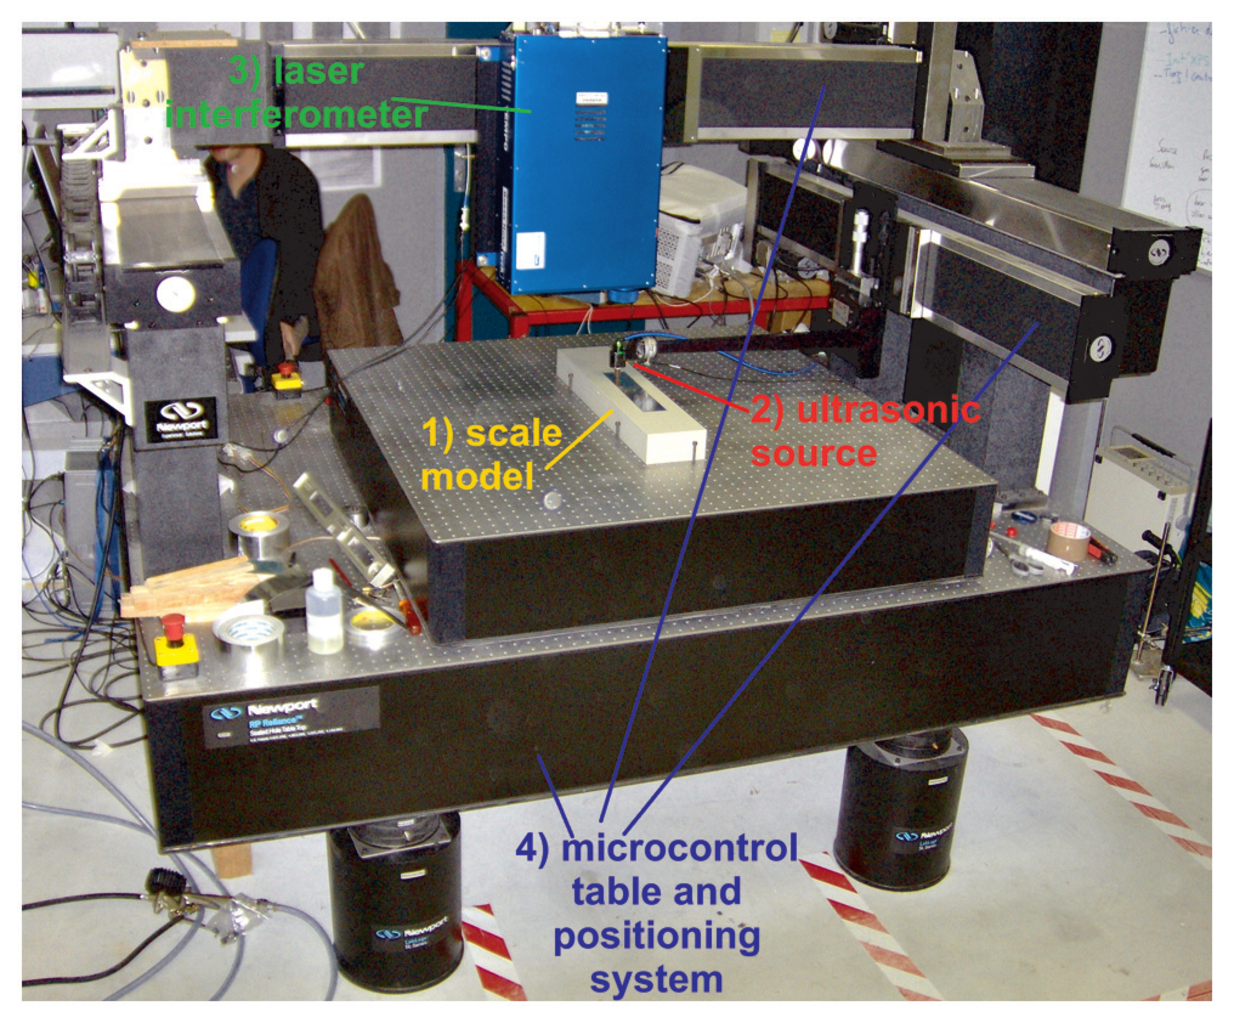
\includegraphics[width=0.50\columnwidth]{Fig/Fig01.eps}
\caption{Photograph of the MUSC ultrasonic laboratory (from \cite{bretaudeau2013fwi} )with its four components: (1) a small-scale model of a subsurface zone, (2) an optical table with two mobile automated arms above the model, (3) a laser interferometer to record ultrasonic wave propagation on the model surface,(4) a piezoelectric ultrasonic source to generate ultrasonic waves in the model.}
\label{Fig:Fig01}
\end{figure}

\clearpage
\newpage

% #### Fig:Fig02
\begin{figure*}
\centering
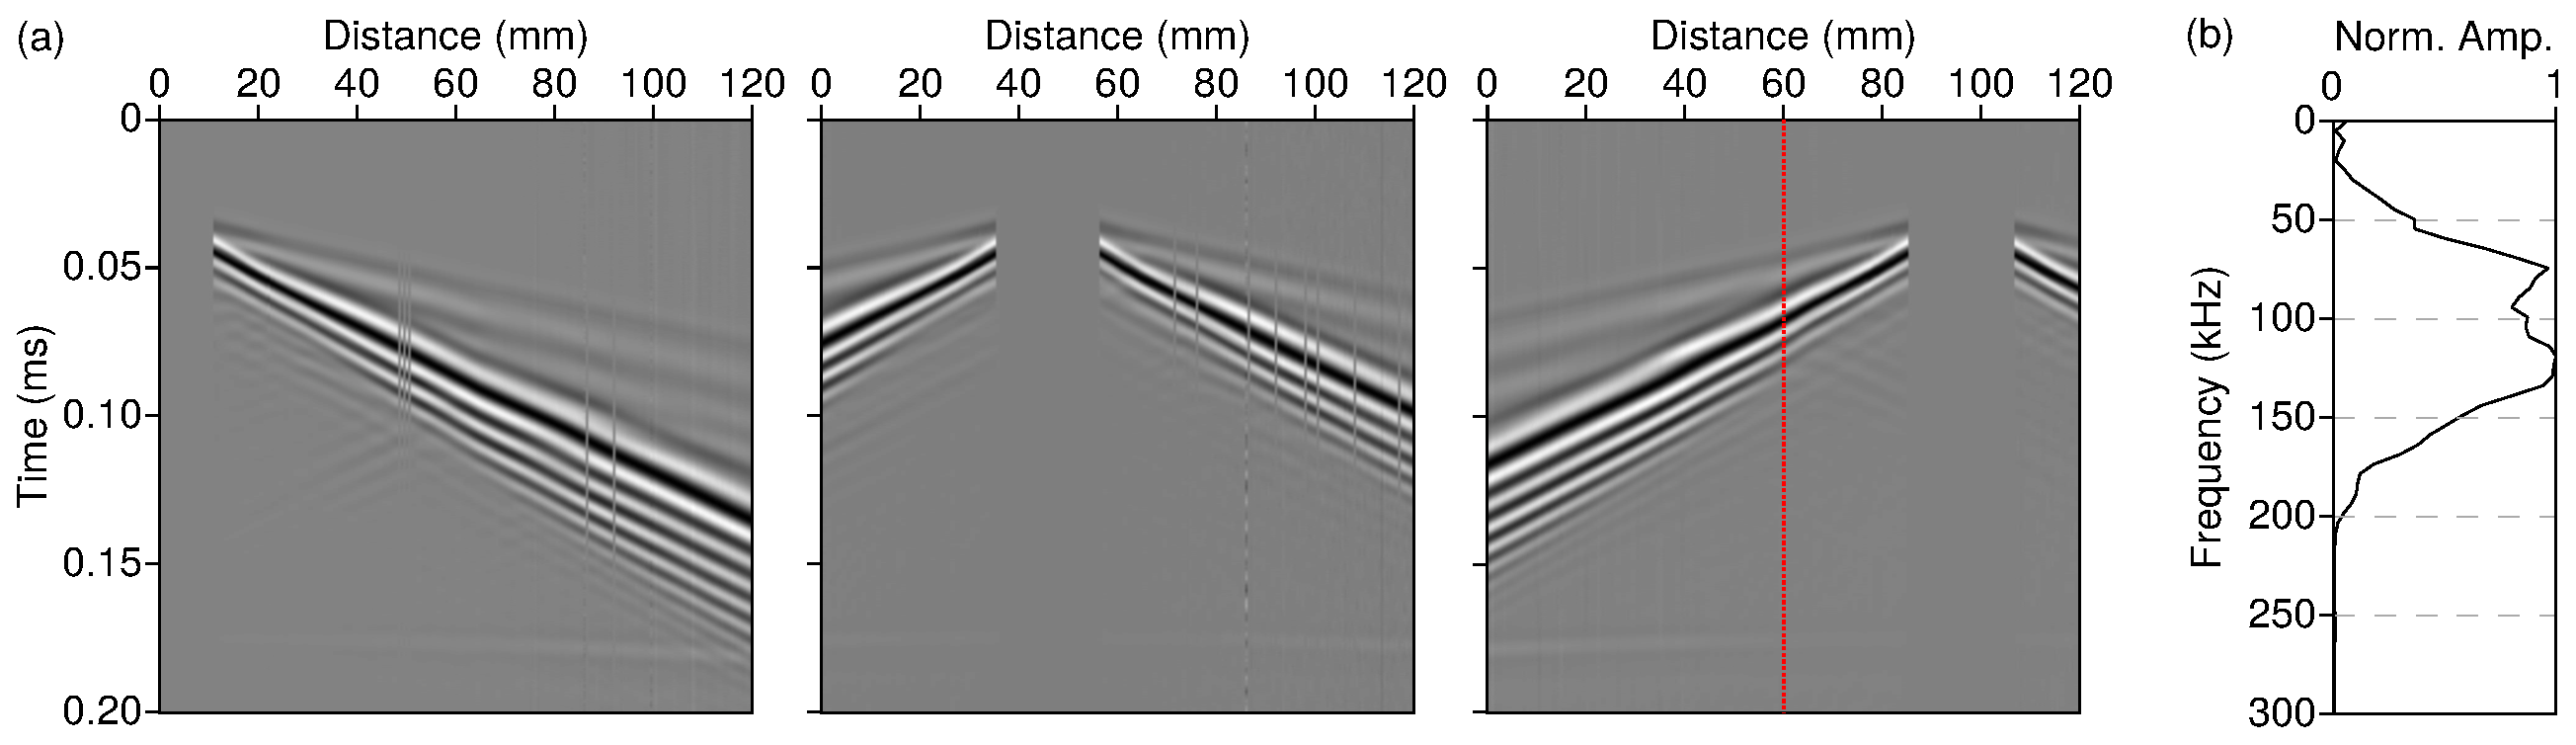
\includegraphics[width=1.00\columnwidth]{Fig/Fig02.eps}
\caption{(a) Examples of multireceiver records in the MUSC laboratory for a two-layer model (\bialt model). Zero-value data correspond to the diameter of the source. (b) Normalized amplitude spectrum of a recorded trace (red line in (a)).}
%\caption{Examples of multireceiver records in the MUSC laboratory for a two-layer model (\bialt model). Zero-value data correspond to the diameter of the source.}
\label{Fig:Fig02}
\end{figure*}

\clearpage
\newpage

% #### Fig:Fig03
\begin{figure}
\centering
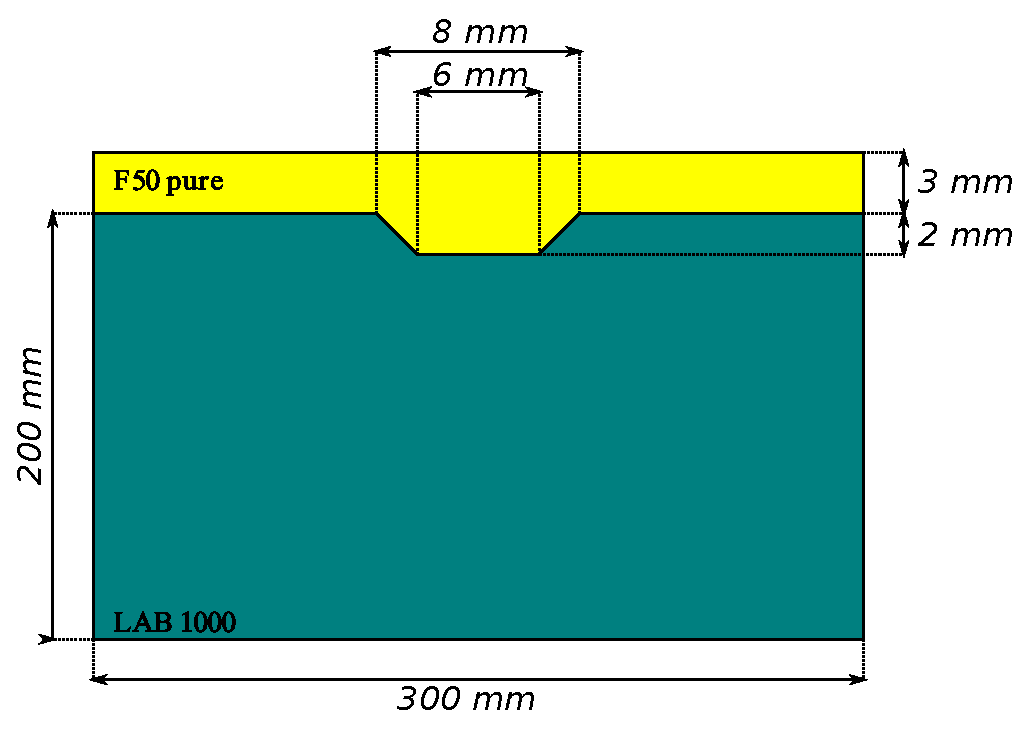
\includegraphics[width=0.50\columnwidth]{Fig/Fig03.eps}
\caption{Schematic representation of (a) the homogeneous model used in this study and (b) the \bialt model.}
\label{Fig:Fig03}
\end{figure}

\clearpage
\newpage

%\begin{figure}
%\centering
%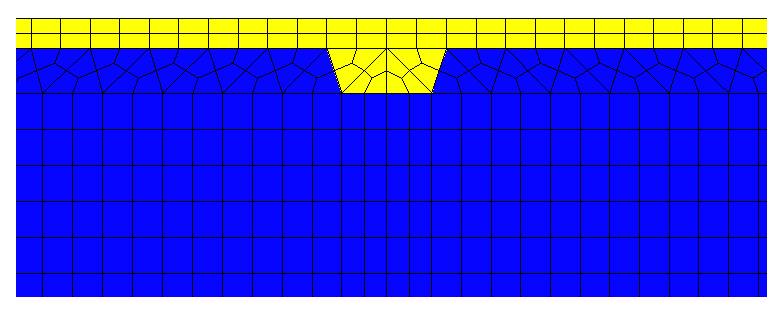
\includegraphics[width=0.50\columnwidth]{Fig/Fig04.eps}
%\caption{Zoom on the mesh of the \bialt model used for numerical modeling.}
%\label{Fig:Fig04}
%\end{figure}

\clearpage
\newpage

% #### Fig:: panel_bialt_2D3D
\begin{figure}
\centering
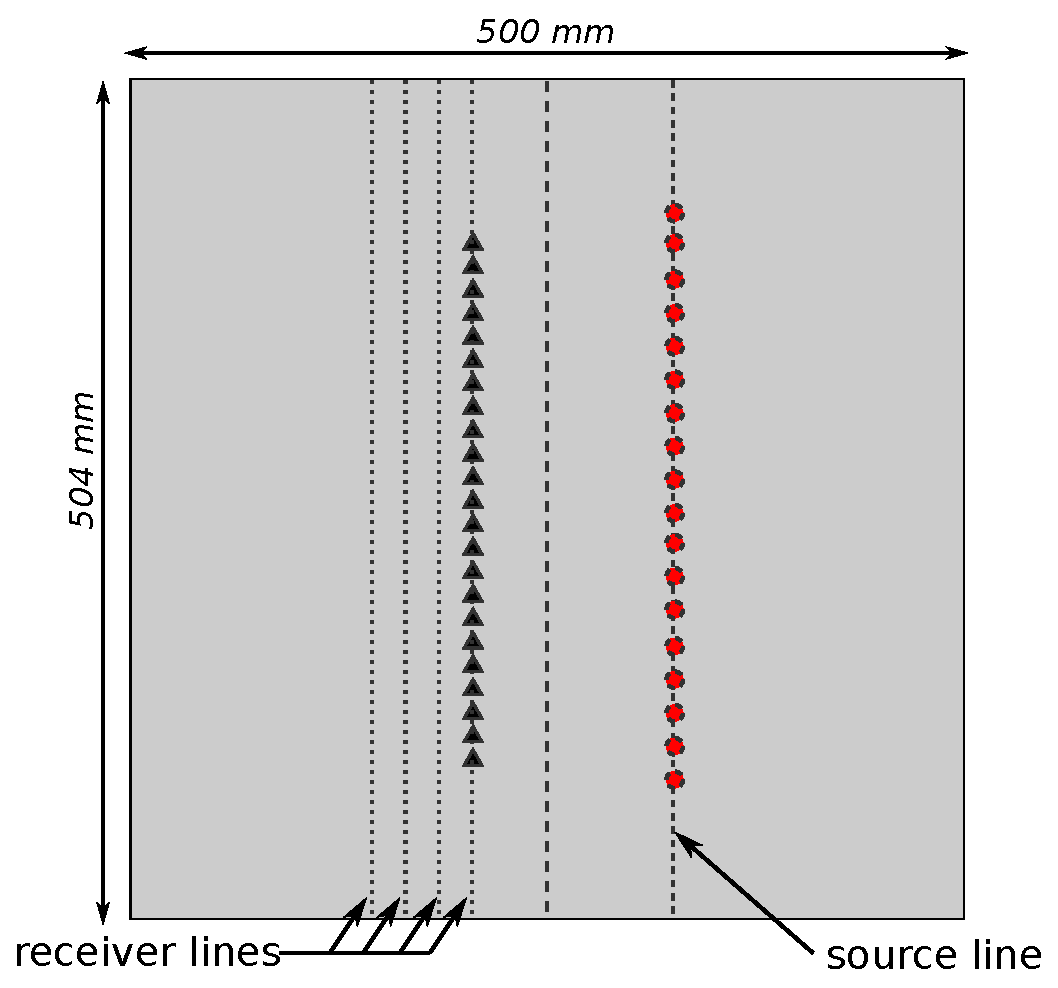
\includegraphics[width=0.50\columnwidth]{Fig/Fig05.eps}
\caption{Schematic representation of the acquisition geometry used to generate an experimental line-source, \textit{i.e.} an equivalent of cylindrical source use in two-dimensional modeling. The black triangles and red circles represent receivers and sources, respectively.}
\label{Fig:Fig05}
\end{figure}

\clearpage
\newpage

\begin{figure*}
\centering
\includegraphics[width=1.0\columnwidth]{Fig/Fig06_new.eps}
\caption{(a,b) Numerical modeling. (a) The resulting seismogram at one receiver position for the experimental line-source. (b) Comparison between 3D point-source response in red (central trace of (a)), 3D constructed line source response of(a) in green and 2D line-source response from 2D modeling in gray. (c,d) the same as (a) and (b) but for experimental modeling.}
\label{Fig:Fig06}
\end{figure*}

\clearpage
\newpage

\begin{figure*}
\centering
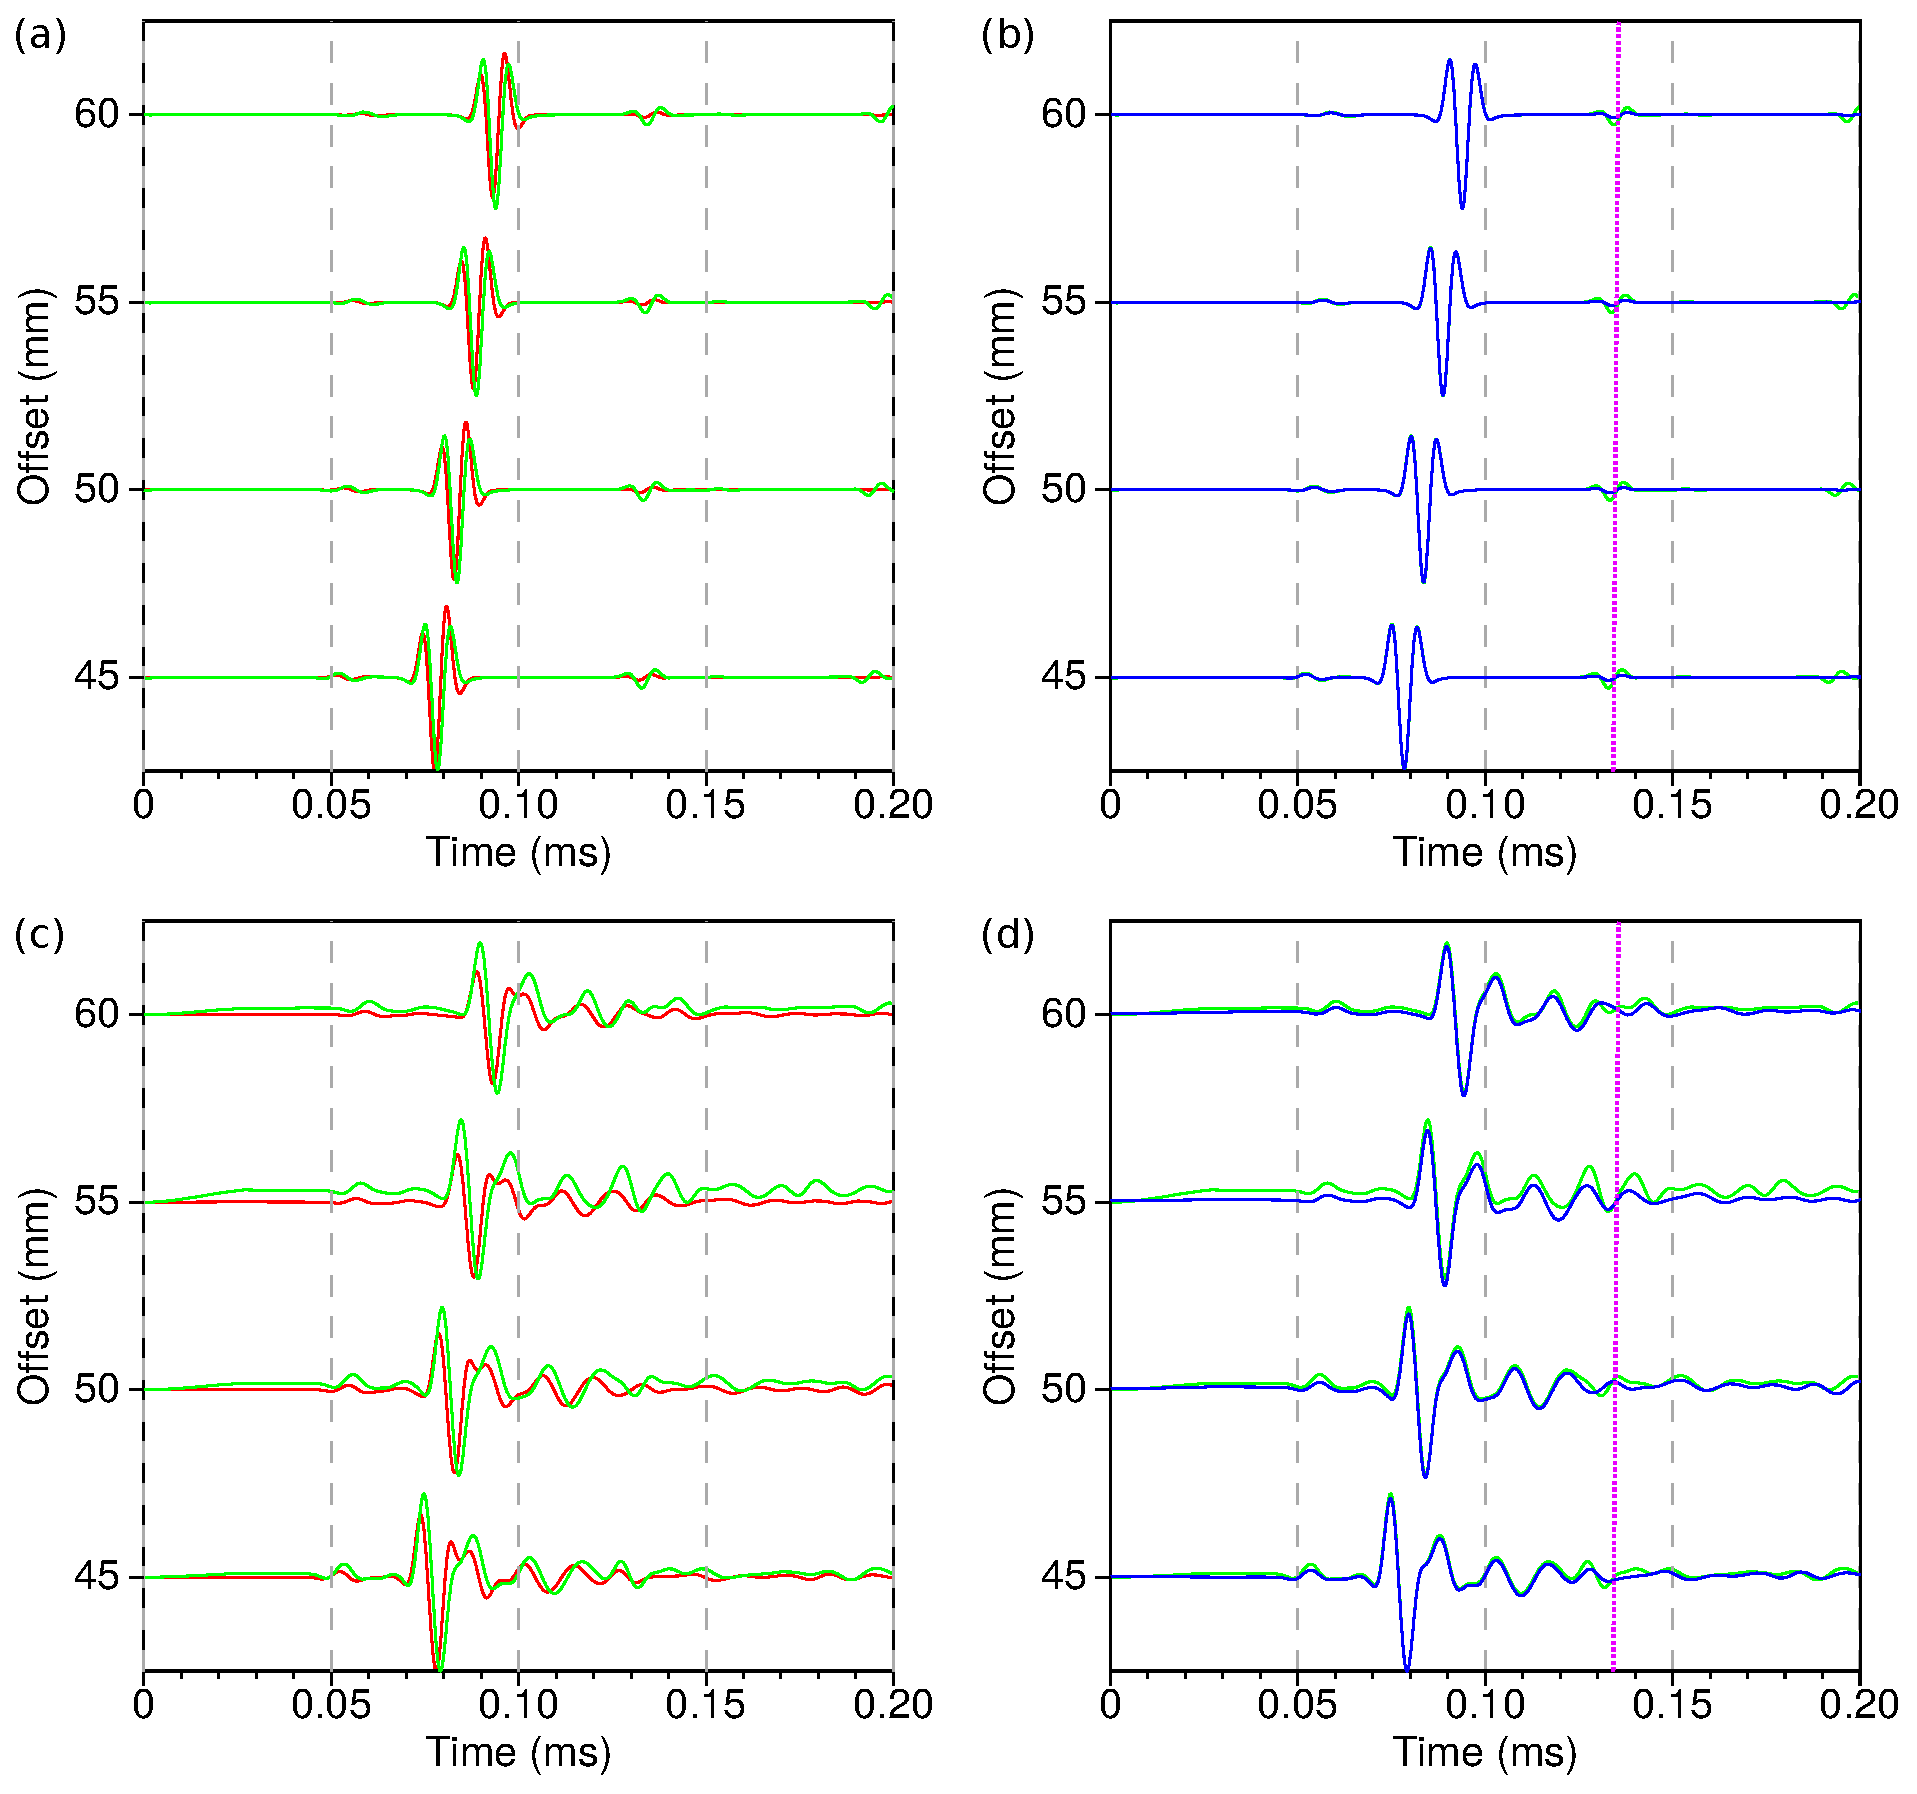
\includegraphics[width=1.0\columnwidth]{Fig/Fig07.eps}
\caption{(a,b) Numerical model. (a) Comparison between synthetic seismograms for a 3D point-source (red) and for a 2D line-source (green), for 45, 50, 55 and 60 mm source-receiver offsets respectively. (b) Comparison between synthetic seismograms for a 2D line-source (green), and a 3D point-source response corrected from geometrical spreading (blue) for the same source-receiver offsets as (a) using the hybrid method with ratios $r=0.35$, $r=0.40$, $r=0.45$ and $r=0.50$ for offsets $45$, $50$, $55$ and $60\ mm$, respectively . (c,d) the same as (a) and (b) for experimental modeling. The light-purple dotted lines depict the peak $PSv$-wavefront.}%\textbf{cc} gives the correlation factor between line-source and point-source responses.}
\label{Fig:Fig07}
\end{figure*}

\clearpage
\newpage

% #### Fig:: panel_srcest_2D_mean
\begin{figure}
\centering
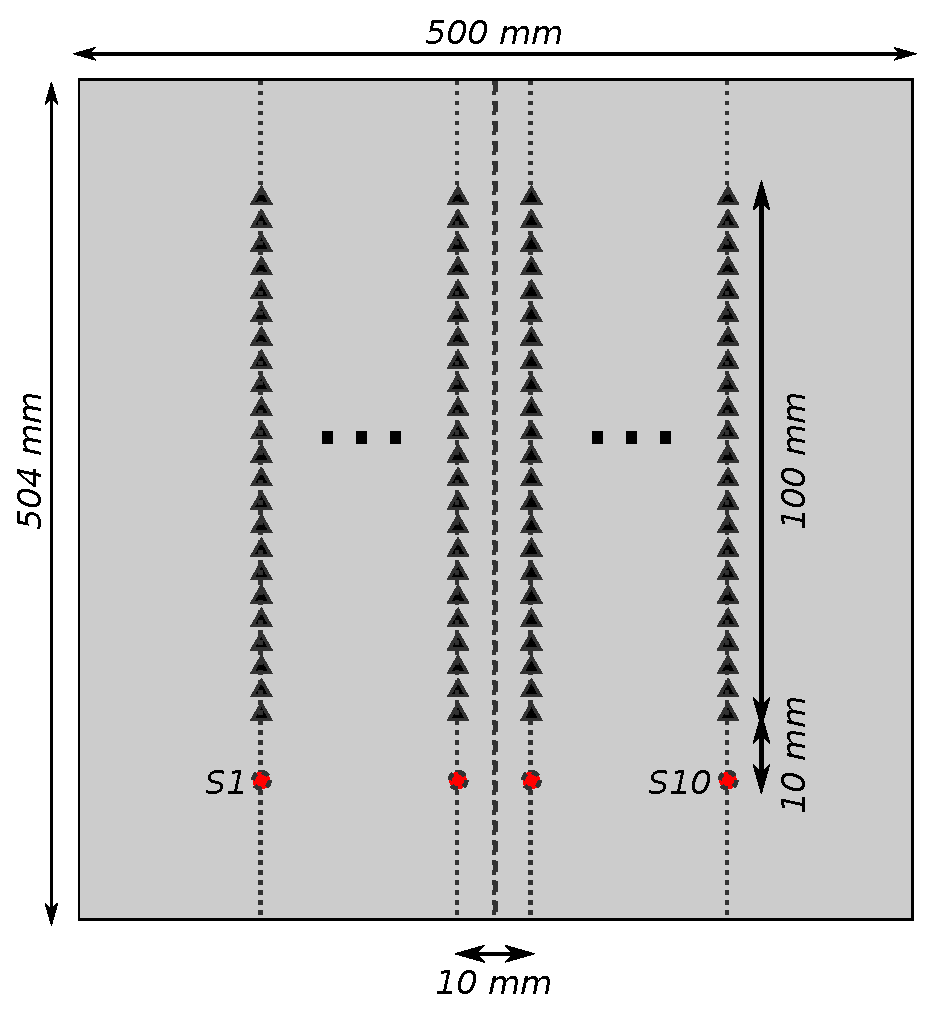
\includegraphics[width=0.50\columnwidth]{Fig/Fig08.eps}
\caption{Schematic representation of the acquisition geometry used to assess data reproducibility using the MUSC laboratory. The black triangles and red circles represent receivers and sources, respectively.}
\label{Fig:Fig08}
\end{figure}

\clearpage
\newpage

\begin{figure}
\centering
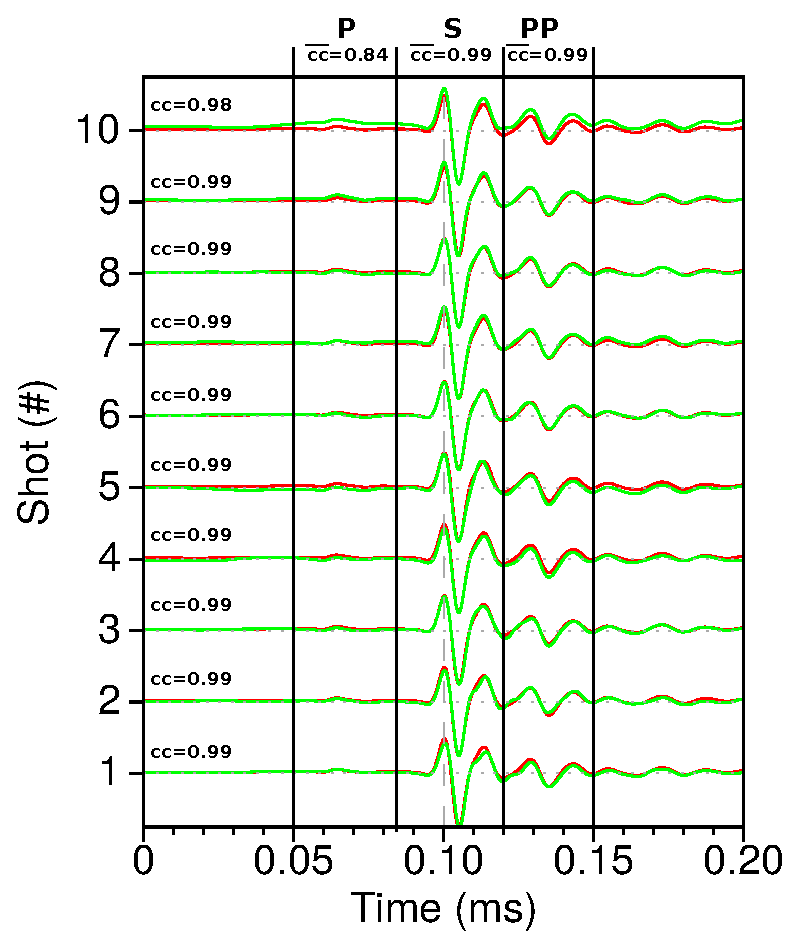
\includegraphics[width=0.50\columnwidth]{Fig/Fig09.eps}
\caption{Central trace for each of the ten analogical experiments compared to a mean central trace (green). $cc$ gives the correlation coefficient between the traces compared for the whole signal while $\overline{cc}$ gives the mean correlation coefficient between the traces compared for a given phase (P, S, PP).}
\label{Fig:Fig09}
\end{figure}

\clearpage
\newpage

\begin{figure}
\centering
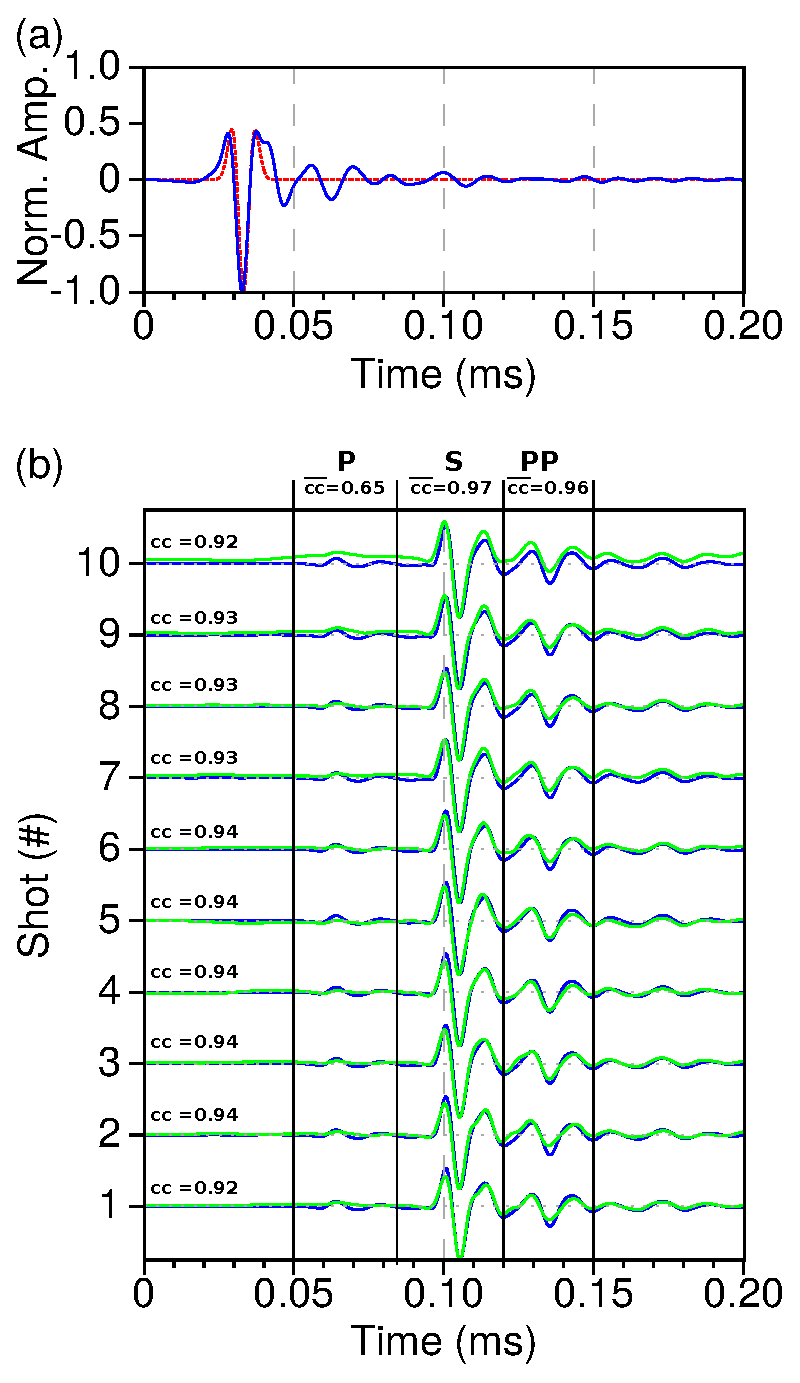
\includegraphics[width=0.50\columnwidth]{Fig/Fig10.eps}
\caption{(a) Comparison between the theoretical Ricker source ($f_{0}=100\ kHz$, $t_{0}=0.03\ ms$) transmitted to the piezoelectric transducer (dashed red line) and the effective source for the homogeneous \textit{F50 pure} model (blue line). (b) Comparison between experimental central and numerical traces using the effective source instead of the theoretical one. $cc$ gives the correlation coefficient between the traces compared for the whole signal while $\overline{cc}$ gives the mean correlation coefficient between the traces compared for a given phase (P, S, PP).}
\label{Fig:Fig10}
\end{figure}

\clearpage
\newpage
% #### Fig:: Fig:Fig03

\begin{figure}
\centering
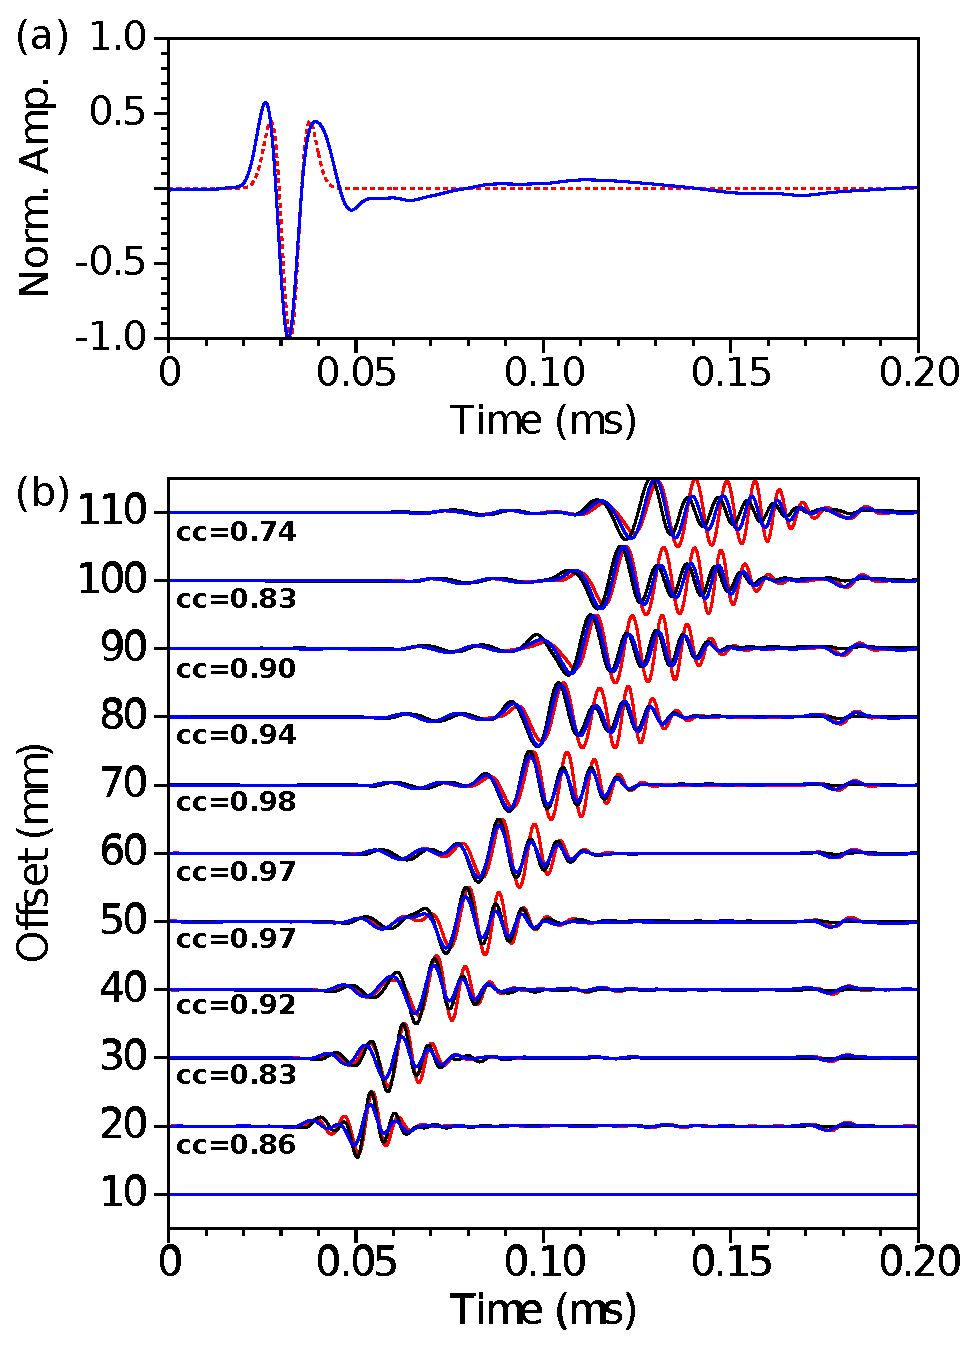
\includegraphics[width=0.50\columnwidth]{Fig/Fig11.eps}
\caption{(a) Comparison between the theoretical Ricker source ($f_{0}=75\ kHz$, $t_{0}=0.03\ ms$) transmitted to the piezoelectric transducer (dashed red line) and the effective source for the \bialt model (blue line). (b) Comparison between experimental central (black) and numerical traces using theoretical source (red) and numerical traces using the effective source (blue). \textbf{cc} gives the correlation coefficient between the traces compared.}
\label{Fig:Fig11}
\end{figure}

\end{document}

